\documentclass[12pt]{article}
\usepackage[brazil]{babel}
\usepackage[utf8]{inputenc}
\usepackage{amsthm,amsfonts,amsmath}
\usepackage[a4paper,margin={1in,1in},vmargin={0.5in,0.5in}]{geometry}
\usepackage{graphicx,color}
\usepackage[font=small,labelfont=bf]{caption}
\usepackage[table,xcdraw]{xcolor}
\usepackage{listings}
\usepackage{verbatim}

\begin{document}
\title{%
    Documentação Trabalho Prático 1 \\
    \vspace{2em}
    \large DCC023 - Redes de Computadores \\
    UNIVERSIDADE FEDERAL DE MINAS GERAIS}

\author{Frederico Ribeiro Queiroz}
\maketitle

\section{Introdução}
O objetivo deste trabalho é implementar um jogo da forca simplificado, jogado entre cliente um
e um servidor, que se comunicam através de \emph{aplicações sockets}. \par
Em um jogo da forca, o jogador deve dar palpites até acertar qual a palavra proposta, sabendo a quantidade de letras presente na mesma.
Será utilizada uma versão simplificada onde os palpites errados não são contabilizados (o jogador não é `enforcado') e o jogo acaba quando todas as letras da palavra são encontradas. \par
Neste jogo, o cliente envia letras como palpites e o servidor recebe e responde os locais de ocorrência da letra, dada que ela exista na palavra.
Os detalhes serão discutidos nas seções seguintes.

\section{Soluções implementadas}
Os programas foram implementados em \emph{linguagem C}. Para realizar a comunicação entre cliente e servidor, foram implementadas aplicações sockets que utilizam o protocolo TCP.
O cliente e o servidor implementados suportam simultâneamente tanto endereços IPv4 quanto IPv6, sem necessidade de alteração em código fonte. 
O detalhe sobre essa interoperabilidade de versão será discutido em uma subseção posterior.\par

\subsection{Protocolo de comunicação}
O protocolo entre cliente e servidor possui quatro tipo de mensagens, da seguinte forma:

\begin{table}[ht]
    \begin{center}
        \begin{tabular}{|c|c|c|c|c|}
            \hline
            \rowcolor[HTML]{FFFFC7}
            \textbf{Mensagem} & \textbf{Descrição} & \multicolumn{3}{c|}{\cellcolor[HTML]{FFFFC7}\textbf{Conteúdo}}                                                         \\ \hline
            Mensagem 1        & Início de jogo     & \begin{tabular}[c]{@{}c@{}}tipo\\ (1 byte)\end{tabular}                                      & \begin{tabular}[c]{@{}c@{}}tamanho da palavra\\ (1 byte)\end{tabular} & \cellcolor[HTML]{C0C0C0}  \\ \hline
            Mensagem 2        & Palpite            & \begin{tabular}[c]{@{}c@{}}tipo\\ (1 byte)\end{tabular}                                      & \begin{tabular}[c]{@{}c@{}}caracter a ser testado\\ (1 byte)\end{tabular} & \cellcolor[HTML]{C0C0C0}  \\ \hline
            Mensagem 3        & Resposta           & \begin{tabular}[c]{@{}c@{}}tipo\\ (1 byte)\end{tabular}                                      & \begin{tabular}[c]{@{}c@{}}número de ocorrências (n)\\ (1 byte)\end{tabular} & \begin{tabular}[c]{@{}c@{}}posições\\ (1 byte * n)\end{tabular} \\ \hline
            Mensagem 4        & Fim de jogo        & \begin{tabular}[c]{@{}c@{}}tipo\\ (1 byte)\end{tabular}                                      & \cellcolor[HTML]{C0C0C0}  & \cellcolor[HTML]{C0C0C0}  \\ \hline
        \end{tabular}
    \end{center}
\end{table}

Por facilidade de implementação, foi criado apenas uma estrutura \emph{(struct MessageInfo)} que contém todos os campos utilizados pelas mensagens.

\newpage
Estrutura criada: 

\begin{center}
    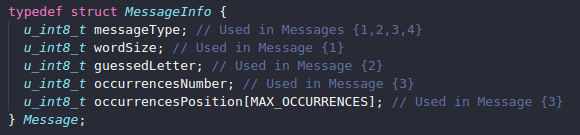
\includegraphics{Figura2.png}
    \captionof{figure}{Estrutura criada para armazenar mensagens}
\end{center}

Dessa forma, foi possível utilizar uma única função \emph{sendMessage()} para enviar e uma \emph{recieveMessage()} para receber mensagens, tanto para o cliente quando para o servidor.
As duas funções e a estrutura da mensagem se encontram na biblioteca comum \emph{src/lib/protocolUtility.h}.

\subsection{Funcionamento básico dos programas}
O esquema a seguir apresenta visualmente o funcionamento básico e o relacionamento dos dois programas:

\begin{center}
    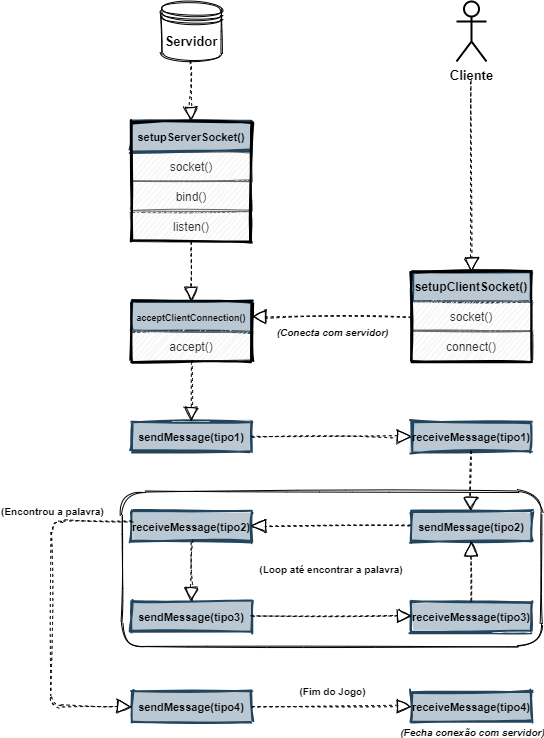
\includegraphics[height=39em]{Figura1.png}
    \captionof{figure}{Funcionamento básico do Servidor e Cliente}
\end{center}

O servidor utiliza a função \emph{setupServerSocket()} para estabelecer um socket.
O cliente utiliza a função \emph{setupClientSocket()} para estabelecer um socket, e em seguida, se conectar ao servidor.
A conexão é aceita pelo servidor através da função \emph{}{acceptClientConnection()}.
A partir desse ponto, servidor e cliente começam a trocar mensagens através das funções \emph{sendMessage()} e \emph{recieveMessage()}
até que o cliente acerta a palavra e receba a mensagem de fim de jogo.

\subsection{Interoperabilidade de versões (IPv4 e IPv6)}
Graças a função \emph{getaddrinfo()} da biblioteca \emph{sys/socket.h} (link para o manual nas referências)
o cliente e o servidor são independentes de versão de IP, inclusive podendo se conectar usando versões distintas (servidor IPv4 e cliente IPv6, por exemplo). \par
A ideia geral é definir argumentos para a \emph{getaddrinfo()} que façam com que ela retorne ambos os endereços (IPv4 e IPv6) e utilize o primeiro endereço que funcione.
Isso é possível graças a uma classe de endereçamento que mapeia ``v4-para-v6''. Os destalhes de implementação dessa função vão além do escopo deste trabalho, portanto serão omitidos. \par

A seguir um exemplo de interoprabilidade entre o servidor e o cliente. \par Neste caso, o servidor está conectado a um endereço IPv4 e solicitaremos a conexão de um cliente passando um endereço IPv6.

\begin{center}
    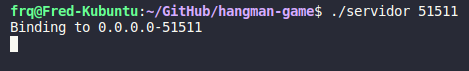
\includegraphics{Figura3.png}
    \captionof{figure}{Servidor conectado a um socket IPv4}
\end{center}

\begin{center}
    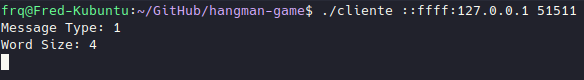
\includegraphics{Figura4.png}
    \captionof{figure}{Cliente conectando com endereço IPv6 se conectando}
\end{center}

\begin{center}
    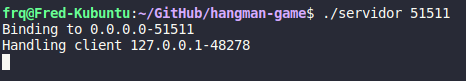
\includegraphics{Figura5.png}
    \captionof{figure}{Servidor recebendo conexão do cliente com endereço IPv4}
\end{center}

O que está acontecendo aqui é que o servidor está `ouvindo' um socket IPv4, e o cliente está tentando conectar utilizando um socket IPv6.
Neste ponto em que o cliente tenta se conectar, o socket ainda não está limitado a um endereço específico, então a implementação do lado do cliente irá reconhecer que está se conectando a um servidor com endereço IPv4
e atribuir um endeço v4 mapeado a partir do endeço v6 ao socket no momento de executar a função \emph{connect()}.

\newpage
\section{Estrutura básica do projeto}


\end{document}